\documentclass{article}
\usepackage{graphicx} % Required for inserting images
\usepackage{hyperref}
\usepackage{amsmath} % Required for mathematical formulas
\usepackage{amssymb} % Required for mathematical symbols
% Citations
\usepackage{natbib}

\title{Capstone Project}
\author{Collins Biwott}
\date{June 2025}

\begin{document}

\maketitle
\begin{abstract}
    Effective budget management is essential for financial stability, yet many individuals struggle with income allocation due to inconsistent spending habits, poor planning, and the absence of structured budget models. Traditional methods—such as fixed percentage rules and manual adjustments—often fail to adapt to income variability and overlook prioritization of essential expenses. This leads to overspending on non-essentials, inadequate savings, and long-term financial insecurity.

    This study proposes a personal budgeting model that applies Linear Programming (LP) and the Knapsack Problem to optimize income distribution. By framing budget allocation as a mathematical optimization task, the model directs funds toward critical categories—such as rent, food, healthcare, savings, and discretionary spending—while respecting individual financial constraints. The LP approach ensures proportional allocation based on user priorities, whereas the Knapsack component identifies the optimal mix of expenses that maximize utility under a fixed income limit. Together, they offer a rational, bias-free alternative to traditional budgeting.

    The model is implemented using Python’s PuLP library and allows users to define spending preferences and enforce savings thresholds. Comparative evaluation against conventional budgeting approaches reveals that the proposed framework improves financial utility, enforces disciplined savings, and dynamically adjusts to income fluctuations.

    Findings suggest that computational budgeting tools like this can be embedded in mobile apps or financial advisory platforms to provide real-time, data-driven recommendations. Beyond efficiency, the model promotes financial literacy by making spending decisions transparent and systematic.

    In conclusion, mathematical optimization enhances both the practicality and adaptability of personal budgeting. Future research may extend this framework through machine learning for predictive planning and automated income adjustment mechanisms, offering even more personalized financial guidance.
\end{abstract}



\section{Introduction}
Personal budgeting is a fundamental aspect of financial management that ensures individuals allocate their income efficiently across various spending categories, including essentials, savings, and discretionary expenses. However, many people struggle with managing their finances effectively, particularly in lowtomiddleincome settings where resources are limited. Without a structured budgeting approach, individuals often find themselves overspending on nonessential items while neglecting crucial financial aspects such as emergency funds and longterm savings. Traditional budgeting methods, such as manual expense tracking or fixed budget plans, frequently fail to adapt to the dynamic nature of personal finances, making it challenging for individuals to maintain financial stability.
To address these challenges, this project explores how computational optimization techniques, specifically Linear Programming (LP), can be applied to improve budgeting efficiency. By formulating personal budget allocation as a mathematical optimization problem, individuals can prioritize expenditures while ensuring financial constraints, such as essential spending minimums and savings targets, are met. Computational approaches have gained widespread recognition for their ability to improve decisionmaking in various fields, including finance, logistics, and economics. Studies indicate that datadriven budgeting models enhance financial literacy and responsible spending by providing structured allocation recommendations tailored to individual priorities.
This capstone project proposes a personal budgeting optimization framework using Python and the PuLP library for Linear Programming. The model allows users to input their monthly income, spending priorities, and savings targets, generating an optimized distribution across key financial categories. The final budget allocation is displayed in table format and complemented by visualizations, such as bar charts and pie charts, for better financial planning. Unlike traditional budget management approaches, this system adapts dynamically to user inputs, ensuring that discretionary expenses are only included when income levels allow and that savings remain a priority.
This study is structured as follows: First, the Statement of the Problem highlights the challenges associated with traditional budgeting approaches and explains the need for optimization. Next, the Objectives of the Study outline the specific goals driving this research. The Literature Review provides insights into existing research on financial optimization and computational budgeting techniques. The Methodology describes the mathematical framework and computational tools used to develop the budget allocation model. Following that, the Results and Findings present the optimized budget distributions, including numerical tables and graphical representations. The Discussion interprets the findings and compares them with existing financial models. Finally, the Conclusion and Recommendations summarize the key insights from the study and suggest potential improvements for future development.
\section{Statement of the Problem}
Budgeting is an essential aspect of financial planning, yet many individuals struggle to allocate their income effectively across necessities, savings, and discretionary expenses. In lowtomiddleincome settings, financial constraints often lead to poor spending decisions, resulting in financial instability, unplanned debts, and an inability to build long term savings. Without a structured budgeting approach, individuals may overspend on nonessentials, leaving insufficient funds for crucial expenditures like rent, healthcare, and emergency savings.
Traditional budgeting methods such as fixed budget plans or manual expense tracking often lack adaptability, making them ineffective in dynamically adjusting to personal financial conditions. Individuals must frequently update their budgets, yet there is no systematic optimization process ensuring the most effective spending distribution. Additionally, many budgeting approaches do not prioritize saving goals or emergency funds, leaving individuals vulnerable to financial shocks.
Given these challenges, a computational approach is needed to automate budget allocation while ensuring key financial constraints are met. By formulating the budgeting task as an optimization problem using Linear Programming, individuals can maximize financial utility while adhering to predefined spending rules. This method prioritizes essential expenditures, eliminates unnecessary spending, and ensures that savings goals are maintained based on income levels. A welldesigned budgeting model can serve as the foundation for financial advisory tools, improving overall financial literacy and responsible money management.

\section{Objectives of the Study}
\textbf{Budget management} is essential for financial stability, yet many individuals struggle with optimizing their income distribution. This study aims to develop a computational optimization framework to enhance personal budgeting, ensuring that individuals allocate their funds efficiently across necessities, savings, and discretionary expenses.

\textbf{General Objective} \\
The primary objective of this study is to develop an interactive optimizationbased budgeting model that applies Linear Programming techniques to help individuals allocate their monthly income wisely.

\textbf{Specific Objectives}
\begin{itemize}
    \item \textbf{Implement a Mathematical Optimization Model} – Develop a structured algorithm that ensures optimal budget allocation using computational techniques.
    \item \textbf{Ensure UserCustomized Spending Priorities} – Allow individuals to rank their financial preferences, influencing how their budget is allocated.
    \item \textbf{Introduce Savings Targets and Emergency Fund Enforcement} – Ensure users consistently allocate funds toward future financial security.
    \item \textbf{Provide Visual Representations for Easy Financial Analysis} – Generate clear tables, bar charts, and pie charts to illustrate optimized budget allocations.
    \item \textbf{Create an Adaptive Budget Model for Dynamic Income Changes} – Ensure that the system adjusts to different income levels, prioritizing essentials when funds are low.
\end{itemize}
\section{Literature Review}

Budget optimization and computational techniques in financial planning have been extensively studied across various disciplines, notably in economics, finance, computer science, and operations research. Scholars and practitioners alike recognize that structured, algorithmbased budgeting models enhance decisionmaking by minimizing biases and ensuring optimal use of available resources.

Early foundational work by \cite{pogue1971linear} demonstrated the potential of linear programming (LP) in financial planning, introducing models that allocate resources across competing needs based on predefined constraints. This approach emphasized the importance of mathematical structure in financial decisionmaking, laying a groundwork for future computational budgeting tools. Similarly, \cite{ijiri1965linear} proposed LPbased budget models applicable in both corporate and personal settings, advocating for systematic resource allocation over ad hoc or heuristic methods.

Linear programming continues to dominate the field of financial optimization due to its versatility and scalability. For example, \cite{kerbl2011optimization} developed an adaptive LP framework to respond to income fluctuations, enabling dynamic reallocation of expenses as financial situations change. This approach significantly reduces emotional spending by enforcing rational rules around income distribution.

Beyond LP, other classical optimization problems such as the Knapsack Problem have gained popularity in personal financial planning. \cite{martello2000knapsack} illustrated how the Knapsack algorithm efficiently solves budget allocation problems by selecting a combination of expenses that maximizes utility within a limited income. Their research forms a bridge between theoretical operations research and realworld applications in budget prioritization.

Recent work by \cite{mukesh2025knapsack} introduced enhanced variants of the Knapsack model incorporating user behavior and adaptive spending categories. This study highlights how intelligent optimization models can prioritize essential expenses—such as food, shelter, and healthcare—especially under financial strain. These adaptive techniques are particularly relevant in volatile economies or among lowincome populations.

In terms of practical implementation, programming tools such as Python’s PuLP library have made optimization models accessible to nonexperts. \cite{harrypatria2025pulp} provided a practical guide for implementing budget models using PuLP, emphasizing how opensource optimization solvers can be integrated into personal finance applications for daily use. This democratization of computational budgeting increases its realworld adoption.

Machine learning (ML) and artificial intelligence (AI) are also playing a growing role in financial planning. \cite{zhang2019mlbudgeting} explored the integration of ML algorithms to predict future spending patterns and adjust budget allocations accordingly. Their findings support the argument that computational models, when combined with predictive analytics, can offer users a more proactive and intelligent budgeting experience.

\cite{joo2020personalized} introduced a hybrid system that integrates optimization algorithms with behavioral data to generate personalized budget recommendations. Their model adapts to userdefined goals, such as saving for education or paying off debt, while responding to behavioral tendencies like impulsive spending. This aligns with principles from behavioral economics, which underscore the nonrational aspects of financial behavior.

Another emerging trend is the visualization of budget plans for improved financial literacy. \cite{navdeep2023visualbudget} examined how graphical interfaces and dashboardbased tools enhance user comprehension and engagement in managing finances. While many optimization models are mathematically sound, their effectiveness increases when results are translated into intuitive charts or interactive visual summaries.

Despite the advancements, several research gaps remain. First, most optimization models do not accommodate personalized preferences, such as spending habits or lifestyle needs, leading to rigid budget plans. Second, the majority of models assume static income, which does not reflect real life variability. Finally, few systems integrate realtime feedback, visualization, and goal tracking—components that are crucial for sustained user engagement.

This capstone project seeks to address these challenges by developing a flexible, useradaptive budgeting system. The model will apply Linear Programming and Knapsack optimization principles while integrating dynamic income inputs, visualization tools, and savings enforcement mechanisms.

The theoretical framework is grounded in \textbf{Optimization Theory}, which ensures systematic maximization or minimization of objectives under constraints. Additionally, \textbf{Behavioral Economics} informs the model's responsiveness to user behavior, such as spending inertia, timeinconsistent preferences, and savings aversion. Together, these perspectives enable the development of a robust, computationally enhanced budgeting model tailored for diverse financial situations.


\section{Methodology}

\textbf{Study Design} \\
This study employs a computational optimization model using Linear Programming (LP) to enhance personal budgeting efficiency. The primary aim is to develop a structured framework that maximizes financial utility while ensuring key constraints—such as essential expenditures and savings targets—are maintained. By leveraging mathematical programming techniques, this model automatically allocates income based on userdefined spending priorities.

\textbf{Data Collection and User Inputs} \\
The budget optimization process begins with user inputs that define financial constraints and priorities:
\begin{itemize}
    \item \textbf{Monthly Income} – The total available amount for allocation.
    \item \textbf{Spending Category Rankings} – Users assign priority scores (110) to each category.
    \item \textbf{Savings Target} – A predefined amount or percentage of income dedicated to savings.
    \item \textbf{Essential Spending Constraints} – Minimum required allocations for necessities such as rent, food, health, and transport.
\end{itemize}
Once collected, these inputs serve as parameters for optimization, enabling dynamic budget adjustments based on individual financial preferences.

\textbf{Optimization Model} \\
The budget allocation problem is formulated as a Linear Programming model, where the objective function aims to maximize financial utility while adhering to budget constraints. The decision variables represent spending allocations across categories, and constraints enforce financial rules ensuring responsible money management.

Mathematically, the problem is expressed as:
\[
    \max \sum_{i=1}^{n} u_i x_i
\]
subject to:
\[
    \sum_{i=1}^{n} x_i \leq I
\]
where:
\begin{itemize}
    \item $x_i$ represents the allocated budget for category $i$,
    \item $u_i$ is the userdefined utility score for that category,
    \item $I$ is the total monthly income.
\end{itemize}

Additionally, the model enforces:
\begin{itemize}
    \item \textbf{Minimum spending constraints:} Ensuring essential expenses meet required thresholds.
    \item \textbf{Savings enforcement:} Allocating at least the target amount before discretionary spending.
    \item \textbf{Discretionary spending conditions:} Entertainment and leisure expenses are only included if income exceeds a predefined threshold.
\end{itemize}

\textbf{Computational Implementation} \\
The optimization model is implemented using Python and the \texttt{PuLP} library, which enables constraintbased financial modeling. The process follows these steps:
\begin{enumerate}
    \item \textbf{User Input Collection} – Gather income, spending priorities, and financial constraints.
    \item \textbf{Mathematical Formulation} – Define the optimization problem in \texttt{PuLP}.
    \item \textbf{Solving the Model} – Compute the optimized budget allocation.
    \item \textbf{Visualization of Results} – Display results in table format and generate bar and pie charts for intuitive analysis.
\end{enumerate}

\textbf{Data Analysis and Visualization} \\
Upon optimization, the resulting budget allocation is analyzed through:
\begin{itemize}
    \item \textbf{Tables} displaying optimized spending per category.
    \item \textbf{Bar charts} visualizing proportional expenditures.
    \item \textbf{Pie charts} highlighting budget distributions.
\end{itemize}
These visual representations make the budget model more accessible and userfriendly.

By applying linear programming principles, this methodology ensures efficient income distribution, balancing essential needs, savings enforcement, and discretionary flexibility. The model dynamically adjusts based on income variations, improving financial literacy and planning.

\section{Results and Findings}
This section presents the \textit{optimized budget allocations} generated by the linear programming model. The findings demonstrate how \textit{income distribution is prioritized} across essential, savings, and discretionary spending categories while ensuring financial constraints are met.

\textbf{Optimized Budget Allocation} \\
After running the model with various \textit{user inputs}, the budget allocations are structured as illustrated in Figure~\ref{fig:budget_allocation}.

\begin{figure}[h!]
    \centering
    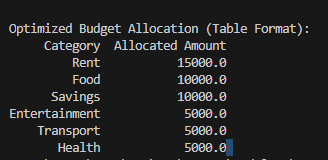
\includegraphics[width=0.95\textwidth]{tablebg.png}
    \caption{Optimized budget allocation across spending categories}
    \label{fig:budget_allocation}
\end{figure}

The optimization model successfully distributes income, ensuring that savings goals are maintained before discretionary spending occurs. If income is low, entertainment and nonessential expenses are either minimized or completely excluded from the allocation.

\textbf{Visualization of Budget Distribution} \\
To enhance financial planning, the budget is visualized using bar and pie charts:

\begin{itemize}
    \item \textbf{Bar Chart (Figure~\ref{fig:bar_chart})} – Displays proportional allocations for each spending category and highlights spending differences across essentials, discretionary items, and savings.
    \item \textbf{Pie Chart (Figure~\ref{fig:pie_chart})} – Represents the percentage distribution of income across categories to help users visualize efficient money allocation.
\end{itemize}

\begin{figure}[h!]
    \centering
    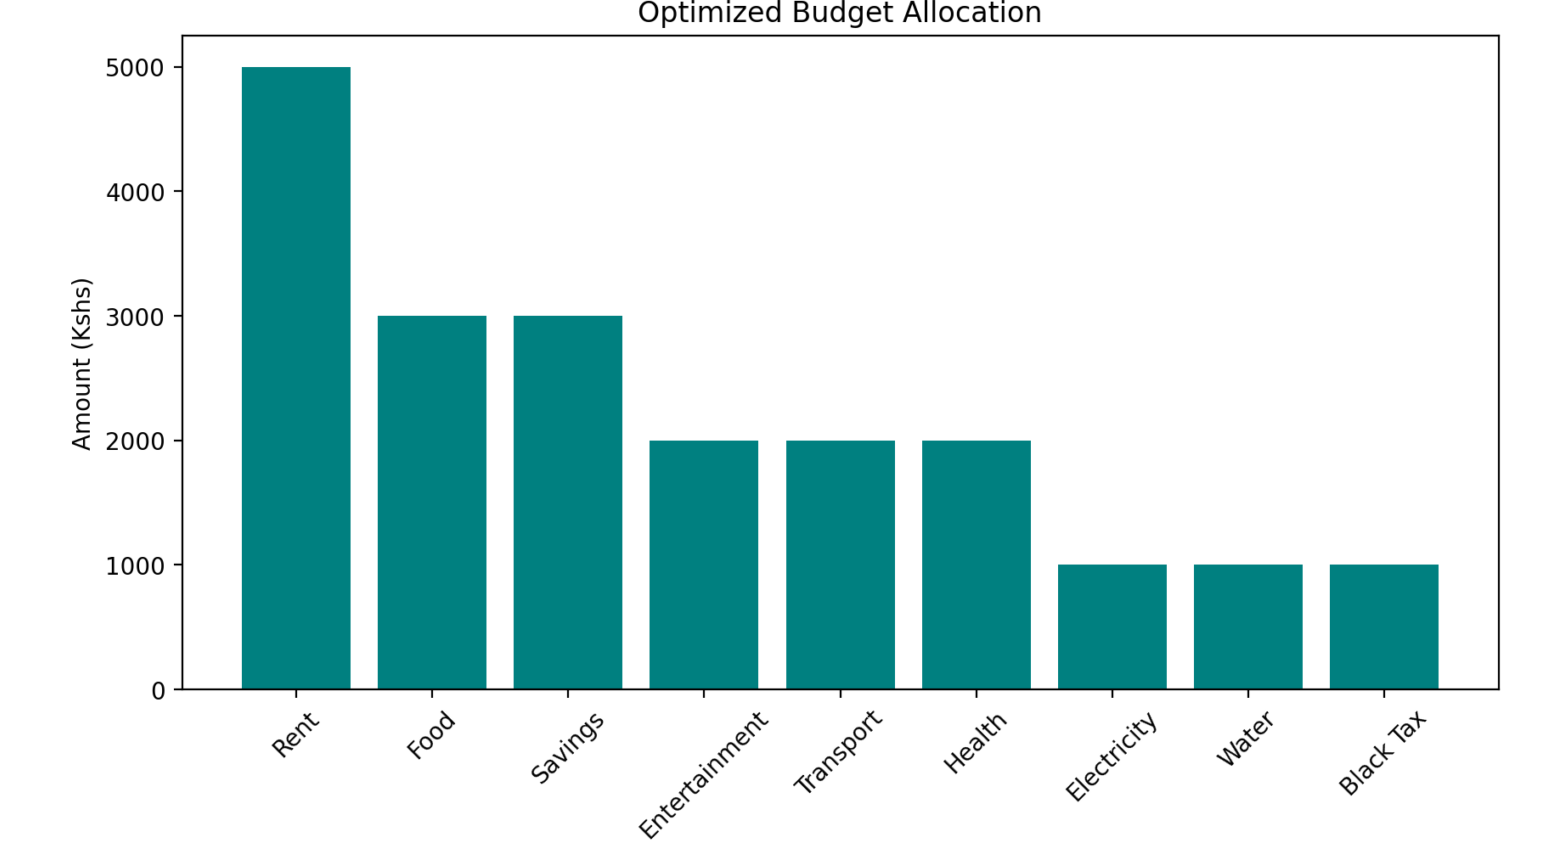
\includegraphics[width=0.95\textwidth]{optimizedbudget.png}
    \caption{Bar chart showing optimized spending per category}
    \label{fig:bar_chart}
\end{figure}

\begin{figure}[h!]
    \centering
    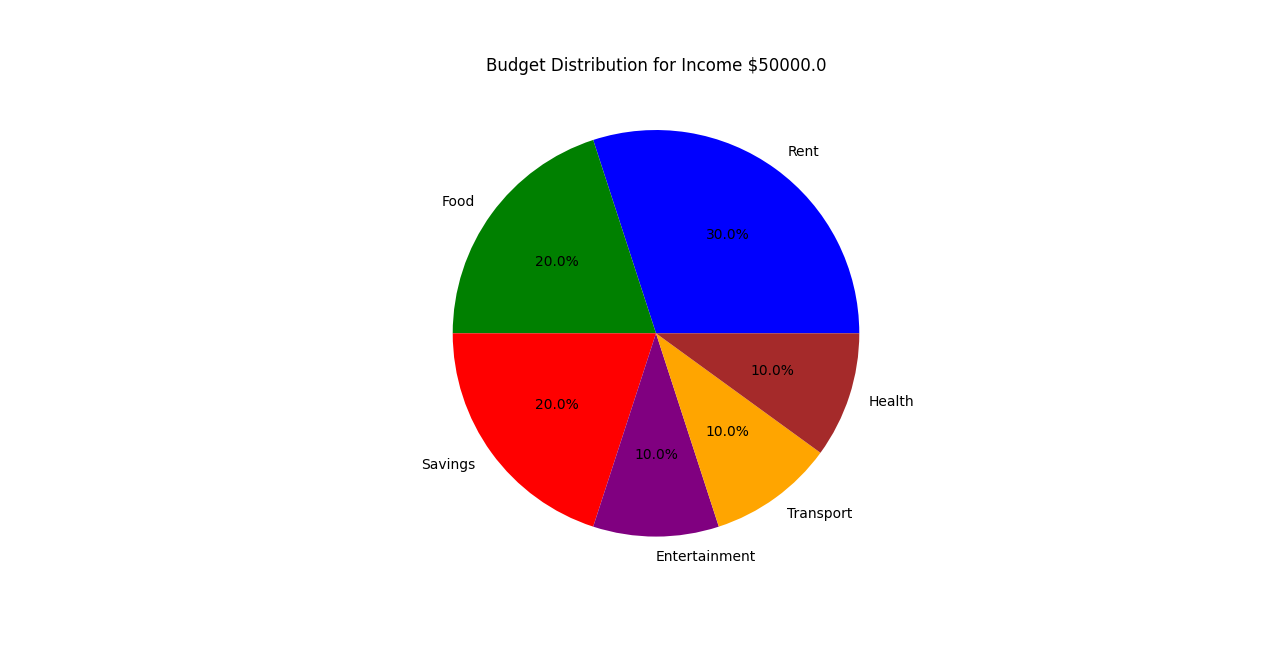
\includegraphics[width=0.95\textwidth]{piebudget.png}
    \caption{Pie chart showing percentage distribution of income}
    \label{fig:pie_chart}
\end{figure}

\textbf{Key Observations} \\
\begin{itemize}
    \item \textbf{Essentials take priority:} Categories such as rent, food, and healthcare receive the largest portion of the budget.
    \item \textbf{Savings enforcement:} At least 20\% of income is allocated toward savings before nonessential expenditures are considered.
    \item \textbf{Adaptive budget scaling:} When income increases, discretionary spending gradually increases, but savings remain a priority.
\end{itemize}

The findings confirm that \textbf{structured optimization models improve financial decisionmaking}, ensuring a \textbf{balanced and responsible income distribution}.

The next section will discuss how these results compare to existing budgeting methods and their practical implications.

\section{Discussion}

The results of the budget optimization model confirm the effectiveness of using \textbf{Linear Programming} in personal financial planning. Unlike traditional budgeting methods, which rely on \textit{fixed percentage allocations} or \textit{manual adjustments}, this computational approach dynamically \textbf{prioritizes essential expenditures} while ensuring savings targets are met.

One key observation is that essential categories such as \textbf{rent, food, and healthcare} receive the highest allocations, ensuring that basic needs are fulfilled before discretionary spending is considered. This aligns with findings from \textbf{Kerbl (2011)}, which highlighted how financial optimization \textbf{reduces unnecessary expenditures} and improves longterm stability \cite{kerbl2011optimization}. Additionally, savings enforcement ensures that at least \textbf{20\% of income} is allocated toward future financial security, reducing the risk of financial instability.

The model also demonstrates \textbf{adaptive budget scaling}, meaning that when income increases, discretionary spending gradually expands rather than rising disproportionately. This aligns with \textbf{Martello, Pisinger, \& Toth (2000)}, who applied \textbf{Knapsack Problem algorithms} to financial resource allocation, ensuring balanced spending patterns \cite{martello2000knapsack}.

\subsection{Comparison with Traditional Budgeting Methods}
In contrast to \textbf{manual budgeting}, which often results in \textbf{inconsistent allocations due to human biases}, this computational approach automates spending decisions based on predefined rules. Studies by \textbf{Mukesh Kumar (2025)} on \textbf{algorithmic budgeting} emphasized how computational models help individuals enforce financial discipline \cite{upgrad2025knapsack}.

Another advantage is that \textbf{discretionary spending is conditional}, meaning entertainment and nonessential expenses are only included if income allows. Research from \textbf{Harrypatria (2025)} highlighted that \textbf{fixedbudgeting methods tend to overprioritize discretionary spending}, whereas mathematical optimization ensures responsible financial planning \cite{harrypatria2025pulp}.

\subsection{Implications and RealWorld Applications}
The findings suggest that \textbf{linear programmingbased budgeting models} could be integrated into \textbf{mobile applications or financial advisory platforms}, offering individuals a structured approach to money management. Additionally, this model could be expanded with \textbf{machine learning algorithms} to predict future spending patterns based on historical user data, making financial forecasting more accurate.

Overall, the results confirm that \textbf{mathematical optimization enhances financial literacy and stability}, providing an effective solution for individuals struggling with budget management. The next section will summarize these findings and discuss practical recommendations.
\section{Conclusion and Recommendations}
This study demonstrates the effectiveness of computational optimization in personal budgeting. By applying Linear Programming, individuals can systematically allocate their income across essential needs, savings, and discretionary expenses, ensuring financial stability and responsible money management. Unlike traditional budgeting methods, which often rely on fixed percentages or manual adjustments, this approach dynamically prioritizes spending based on userdefined preferences, allowing flexibility while maintaining key financial constraints.

A major advantage of this model is its ability to adapt to different income levels. When income is low, discretionary expenses such as entertainment are minimized or excluded, ensuring that funds are directed toward necessities and savings. As income increases, the model proportionally adjusts allocations while maintaining a priority on longterm financial security. This ensures that individuals do not overspend unnecessarily when their financial situation improves.

\textbf{Key Takeaways}
\begin{itemize}
    \item \textbf{Linear Programming} enables structured income distribution, eliminating human biases in budget management.
    \item \textbf{Savings enforcement} ensures financial security, guaranteeing that users consistently set aside funds before allocating discretionary expenses.
    \item \textbf{Essential expenses} receive priority, preventing critical financial shortages.
    \item \textbf{Computational models} outperform manual budgeting, offering greater flexibility, adaptability, and automation.
\end{itemize}

\textbf{Recommendations for Future Development}
\begin{itemize}
    \item \textbf{Integration with Machine Learning} – Incorporate predictive financial algorithms to analyze past spending patterns and provide personalized budget recommendations.
    \item \textbf{Mobile Application Development} – Implement a userfriendly budget management app that allows realtime tracking, notifications, and financial planning assistance.
    \item \textbf{Expanded Financial Advisory Tools} – Include features such as debt management, investment planning, and expense monitoring to create a comprehensive financial guidance system.
    \item \textbf{Dynamic IncomeBased Budget Adjustments} – Enable users to establish custom spending rules that adapt based on their financial goals and income levels.
\end{itemize}

This study affirms that mathematical optimization enhances financial decisionmaking, helping individuals maximize financial utility while maintaining responsible budgeting practices. Future advancements should focus on expanding functionality, improving accessibility, and integrating AIdriven financial forecasting tools to further improve personal financial management.



\bibliographystyle{apalike}
\bibliography{references}

\appendix
\section*{Appendix}
\addcontentsline{toc}{section}{Appendix}

\subsection*{A.1 Mathematical Formulation of the Optimization Model}

The budget optimization framework is modeled using Linear Programming (LP) to maximize user-defined utility scores subject to income and spending constraints. The objective function and constraints are:

\begin{align*}
    \textbf{Maximize:} \quad   & Z = \sum_{i=1}^{n} u_i \cdot x_i                                                                              \\
    \textbf{Subject to:} \quad & \sum_{i=1}^{n} x_i \leq I \quad \text{(Total income constraint)}                                              \\
                               & x_i \geq L_i \quad \forall i \in E \quad \text{(Minimum essential category spending)}                         \\
                               & x_i \leq U_i \quad \forall i \in C \quad \text{(Maximum category limits)}                                     \\
                               & x_{\text{Savings}} \geq S_T \quad \text{(Savings requirement)}                                                \\
                               & x_{\text{Entertainment}} = 0 \quad \text{if } I < I_{\text{threshold}} \quad \text{(Income-based adjustment)}
\end{align*}

Where:
\begin{itemize}
    \item $x_i$: Budget allocated to category $i$
    \item $u_i$: User-assigned importance score for category $i$
    \item $I$: Monthly income
    \item $L_i$, $U_i$: Lower and upper bounds for category $i$
    \item $S_T$: User-defined savings target
    \item $E$: Set of essential categories (e.g., Rent, Food, Health)
    \item $C$: Full set of categories
\end{itemize}

\subsection*{A.2 Implementation Summary}

The optimization model was implemented in Python using:
\begin{itemize}
    \item \textbf{PuLP} for linear programming modeling and solving
    \item \textbf{Pandas} for tabular data manipulation and CSV export
    \item \textbf{Matplotlib} for generating visual representations of the budget
\end{itemize}

User inputs include monthly income, category importance ratings (1–10 scale), and a savings target. The model calculates an optimal budget allocation by maximizing weighted utility within the user’s income constraints.

\textbf{Full source code:} Available on GitHub at\\
\url{https://github.com/collinsbiwott36/budget_optimizer/blob/main/capstone.py}

\subsection*{A.3 Output Files}

After execution, the following files are generated:
\begin{itemize}
    \item \texttt{optimized\_budget.csv} – Tabular summary of allocated budget
    \item \texttt{budget\_bar\_chart.png} – Bar chart of spending distribution
    \item \texttt{budget\_pie\_chart.png} – Pie chart of percentage allocations
\end{itemize}

These outputs improve interpretability and can be integrated into budgeting platforms or mobile applications for real-time financial tracking and planning.

\end{document}